%!TEX root = ../MasterThesis.tex

\chapter{Concept and Design of the System} % (fold)
\label{cha:design_system}
\todo{ca. 30 pages}

\begin{figure}[H]
	\centering
		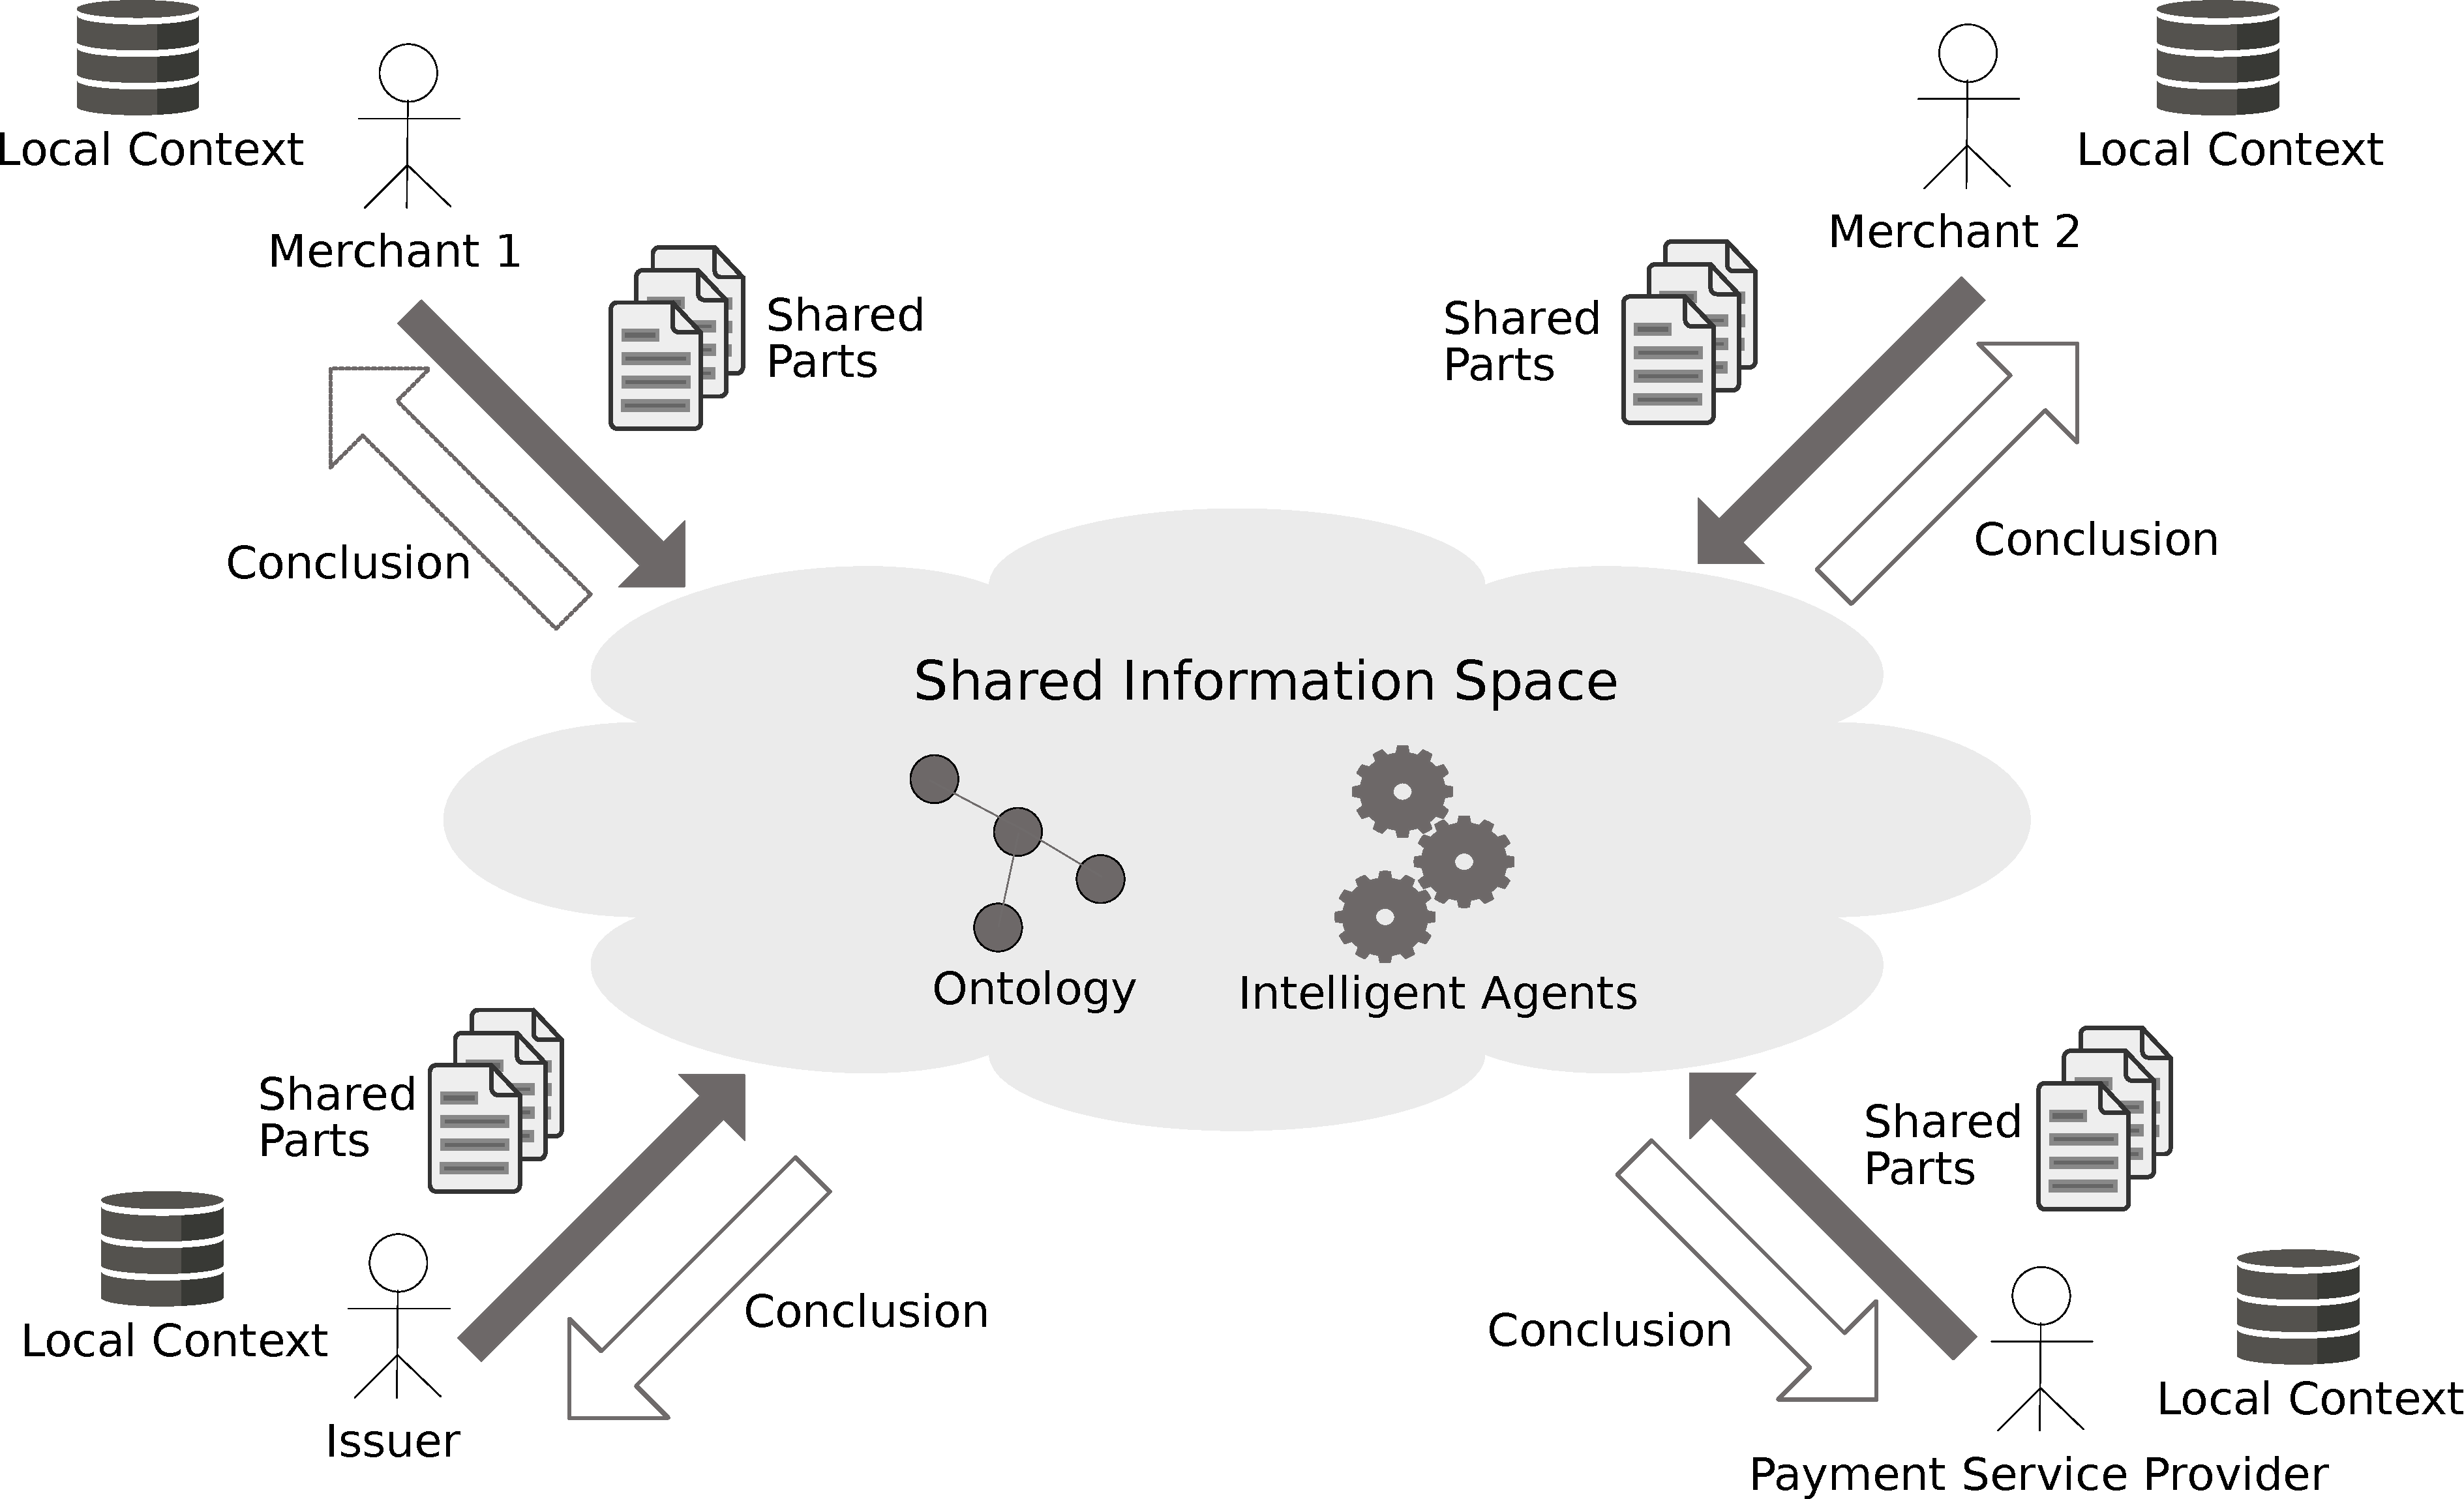
\includegraphics[width=0.8\columnwidth]{images/system_overview.pdf}
	\caption{System Overview}
\label{fig:images_system_overview}
\end{figure}

Based on chapter \ref{sec:cscw} we can conclude: \\
1. Face-to-Face Meetings: out-of-scope of this thesis \\
2. Distance Meetings: lack of collaboration support \\
3. Continuous Tasks: collaboration in teams, but only works when everyone is online \\
4. Communicate \& Collaborate: allows to work on it in a disconnected mode, but increases
communication and coordination efforts as well as might lead to synchronisation issues over time \\
\\
This either leaves us with two options: \\
1. build a distributed, synchronous collaboration system, in that ppl. can share and work on content at the same time \\
2. build a distributed, asynchronous collaboration and communication system, in that ppl. can work on things for themselves and
get connected together at a certain point in time for synchronising their findings and develop new insights \\
\\
In the first variant it can be assumed that: \\
- stakeholders will initiate a collaborative session for a certain case, the collaboration and information sharing efforts end
with finishing the case. \\
- each stakeholder might just work on his part of expertise in the whole knowledge graph (e.g. named subgraphs per stakeholder).
these parts could be easily mirrored on the stakeholders environment (no discrepancies with informations from others) \\
- the whole knowledge graph is only available during the p2p collaboration session, nevertheless results and findings (per stakeholder?)
can be synchronized into the named graph of the stakeholder and be analysed offline \\
- \ldots \\
\\
In the second variant it can be assumed that: \\
- every stakeholder holds different parts of the whole knowledge graph, even might hold the whole graph on his machine. \\
- stakeholders can fill out the information offline, they might get together at irregular intervals to synchronise their efforts and
come up with new knowledge graph entries based on the work of the others \\
- during the synchronisation process there might come up discrepancies due to the different understandings of the stakeholders for a certain aspect of
the knowledge graph \\
- there might also be different findings or result, even contradictory statements, based on the different progress of each stakeholder on the knowledge graph \\
- \ldots \\
\\

Based on chapter \ref{sec:semantic_models} we might come up with a design of the shared information space that looks like this: \\

\begin{figure}[H]
	\centering
		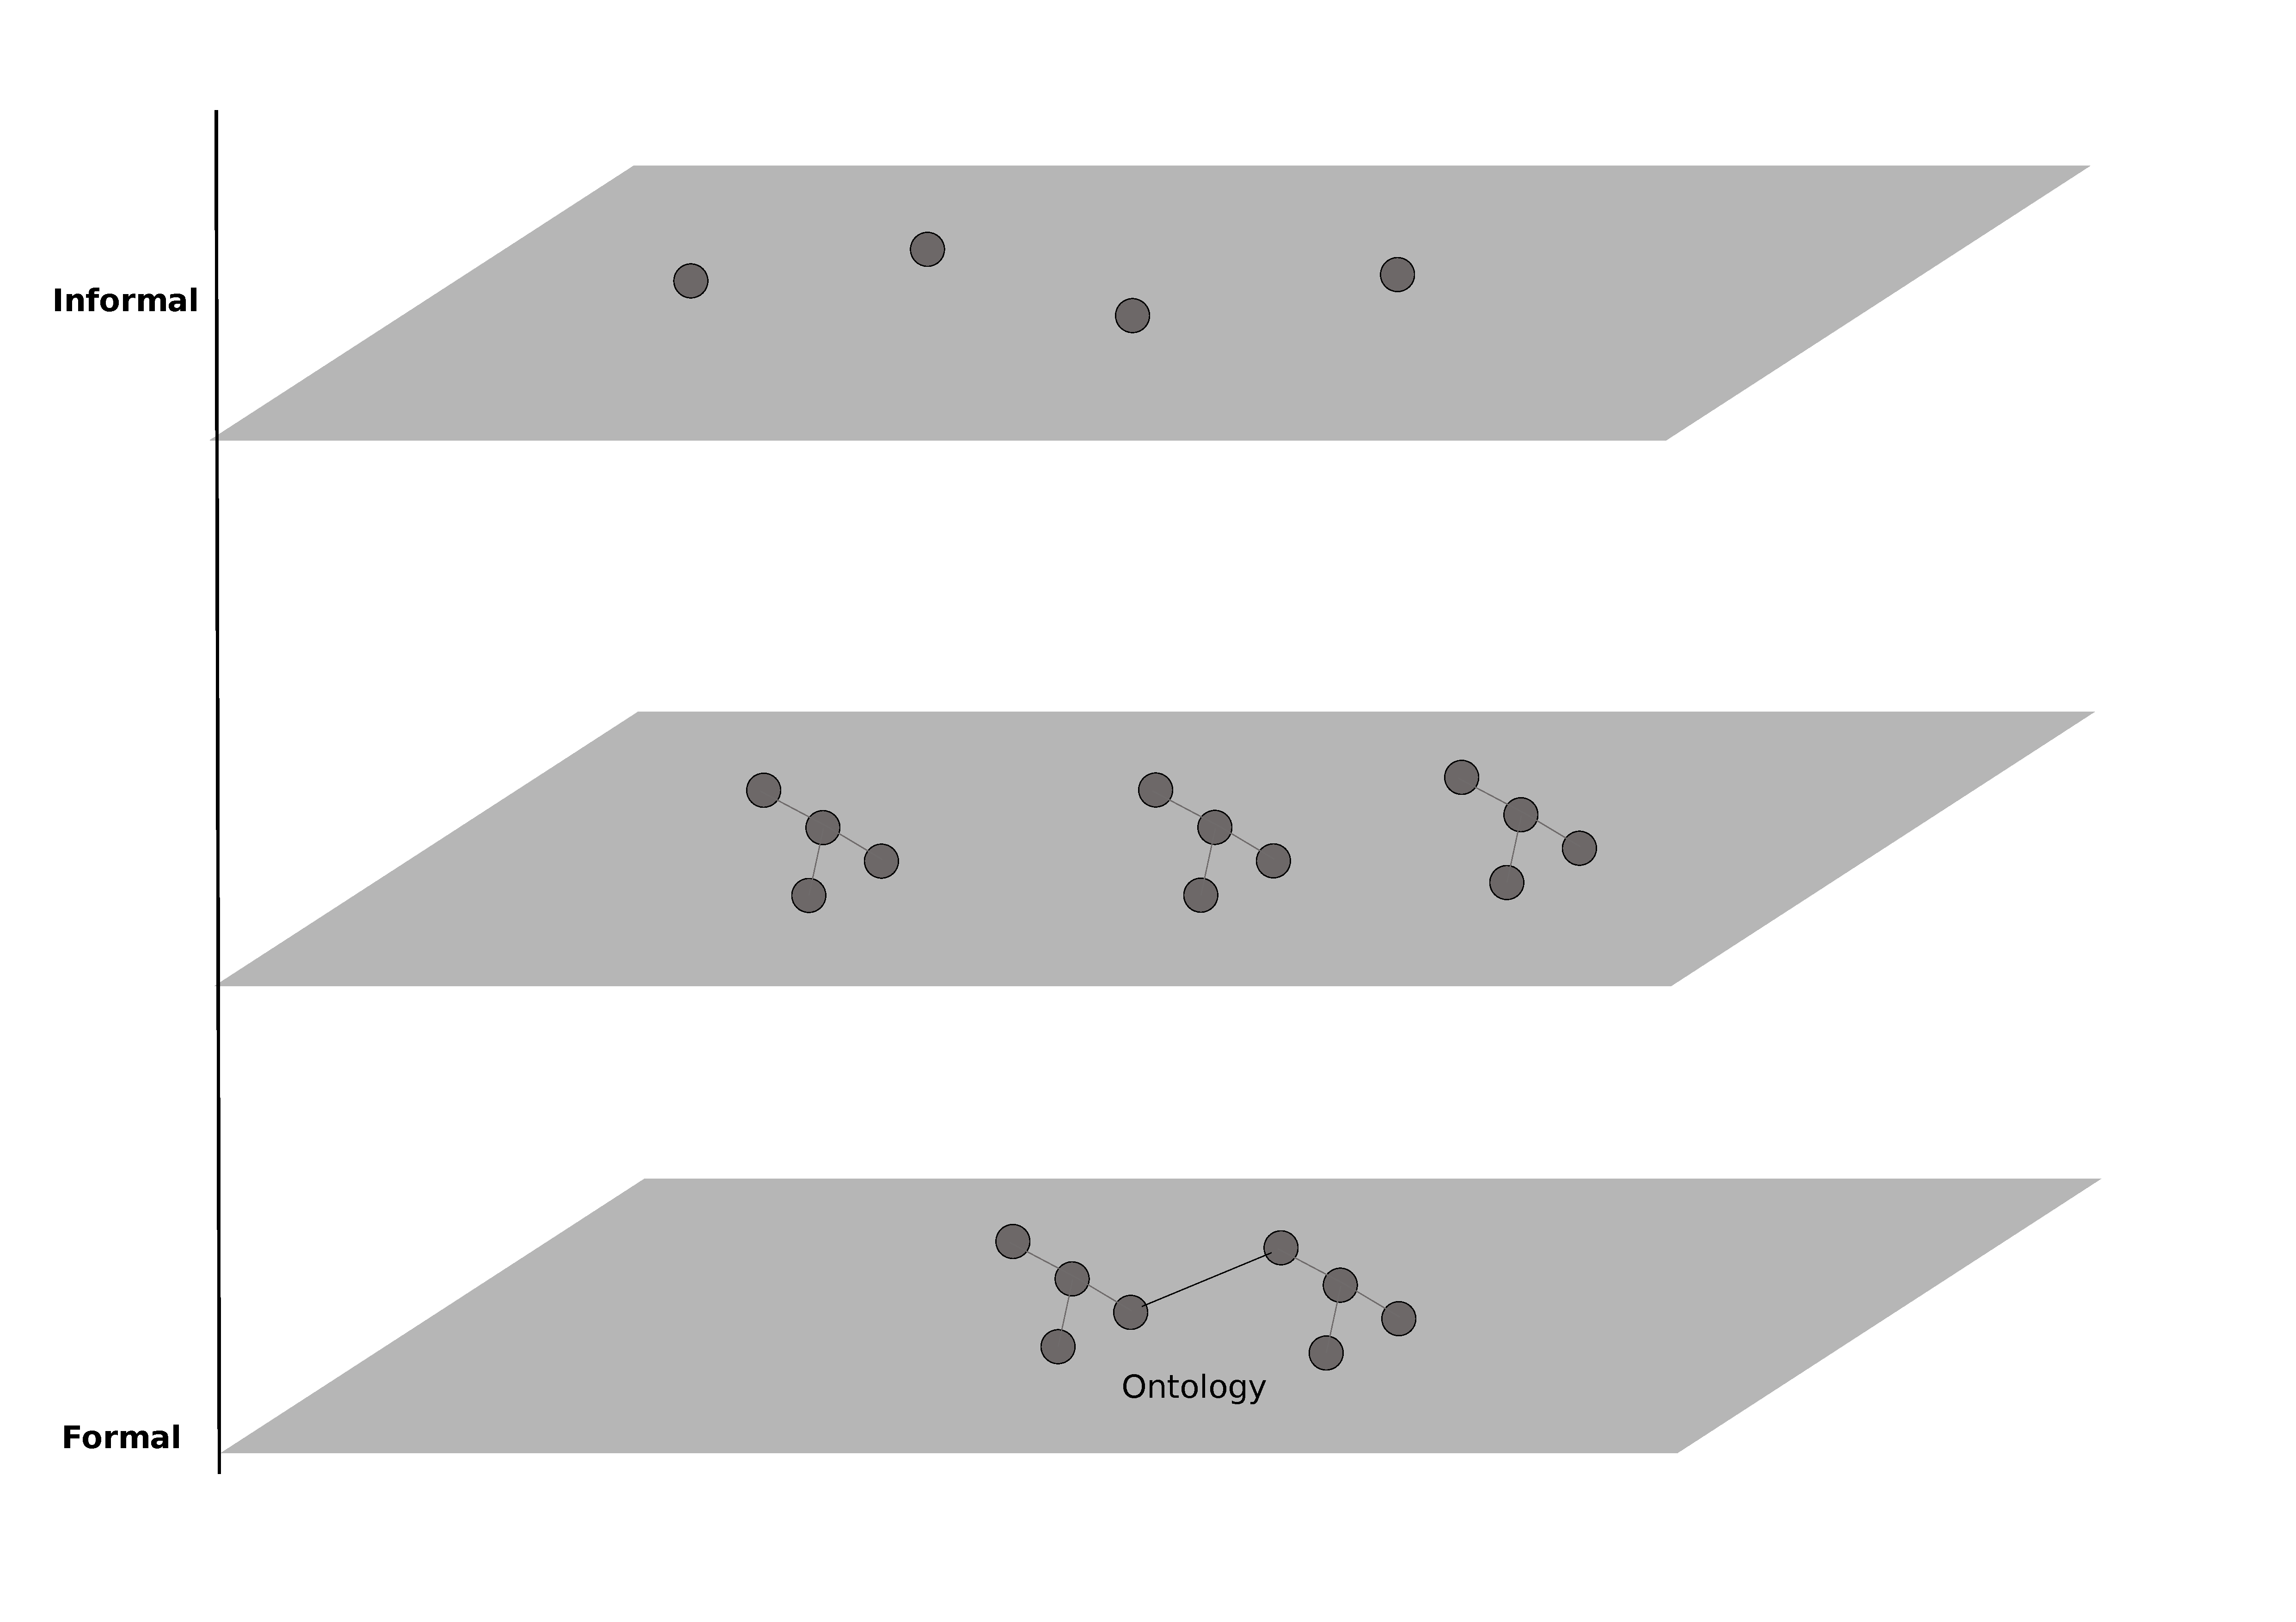
\includegraphics[width=0.8\columnwidth]{images/sharedspace_layers.pdf}
	\caption{Shared Information Space}
\label{fig:images_sharedspace_layers}
\end{figure}

- it uses different layers to connect domain specific knowledge \\
- these layers are ordered based on formalism and models available \\
- the more informal a layer is the more collaboration is required to come up with a shared understanding / the common sense
and connect it with the layer below \\
- layers can be easily turned on / off in the application to focus on a specific aspect of the investigation \\
\\

Based on chapter \ref{sec:p2p_communication} we can either do: \\
- a partially centralized P2P system: having the supernodes that hold the information about the participating parties as well as the
whole graph for analyses at trustworthy parties like the BKA \\

\begin{figure}[H]
	\centering
		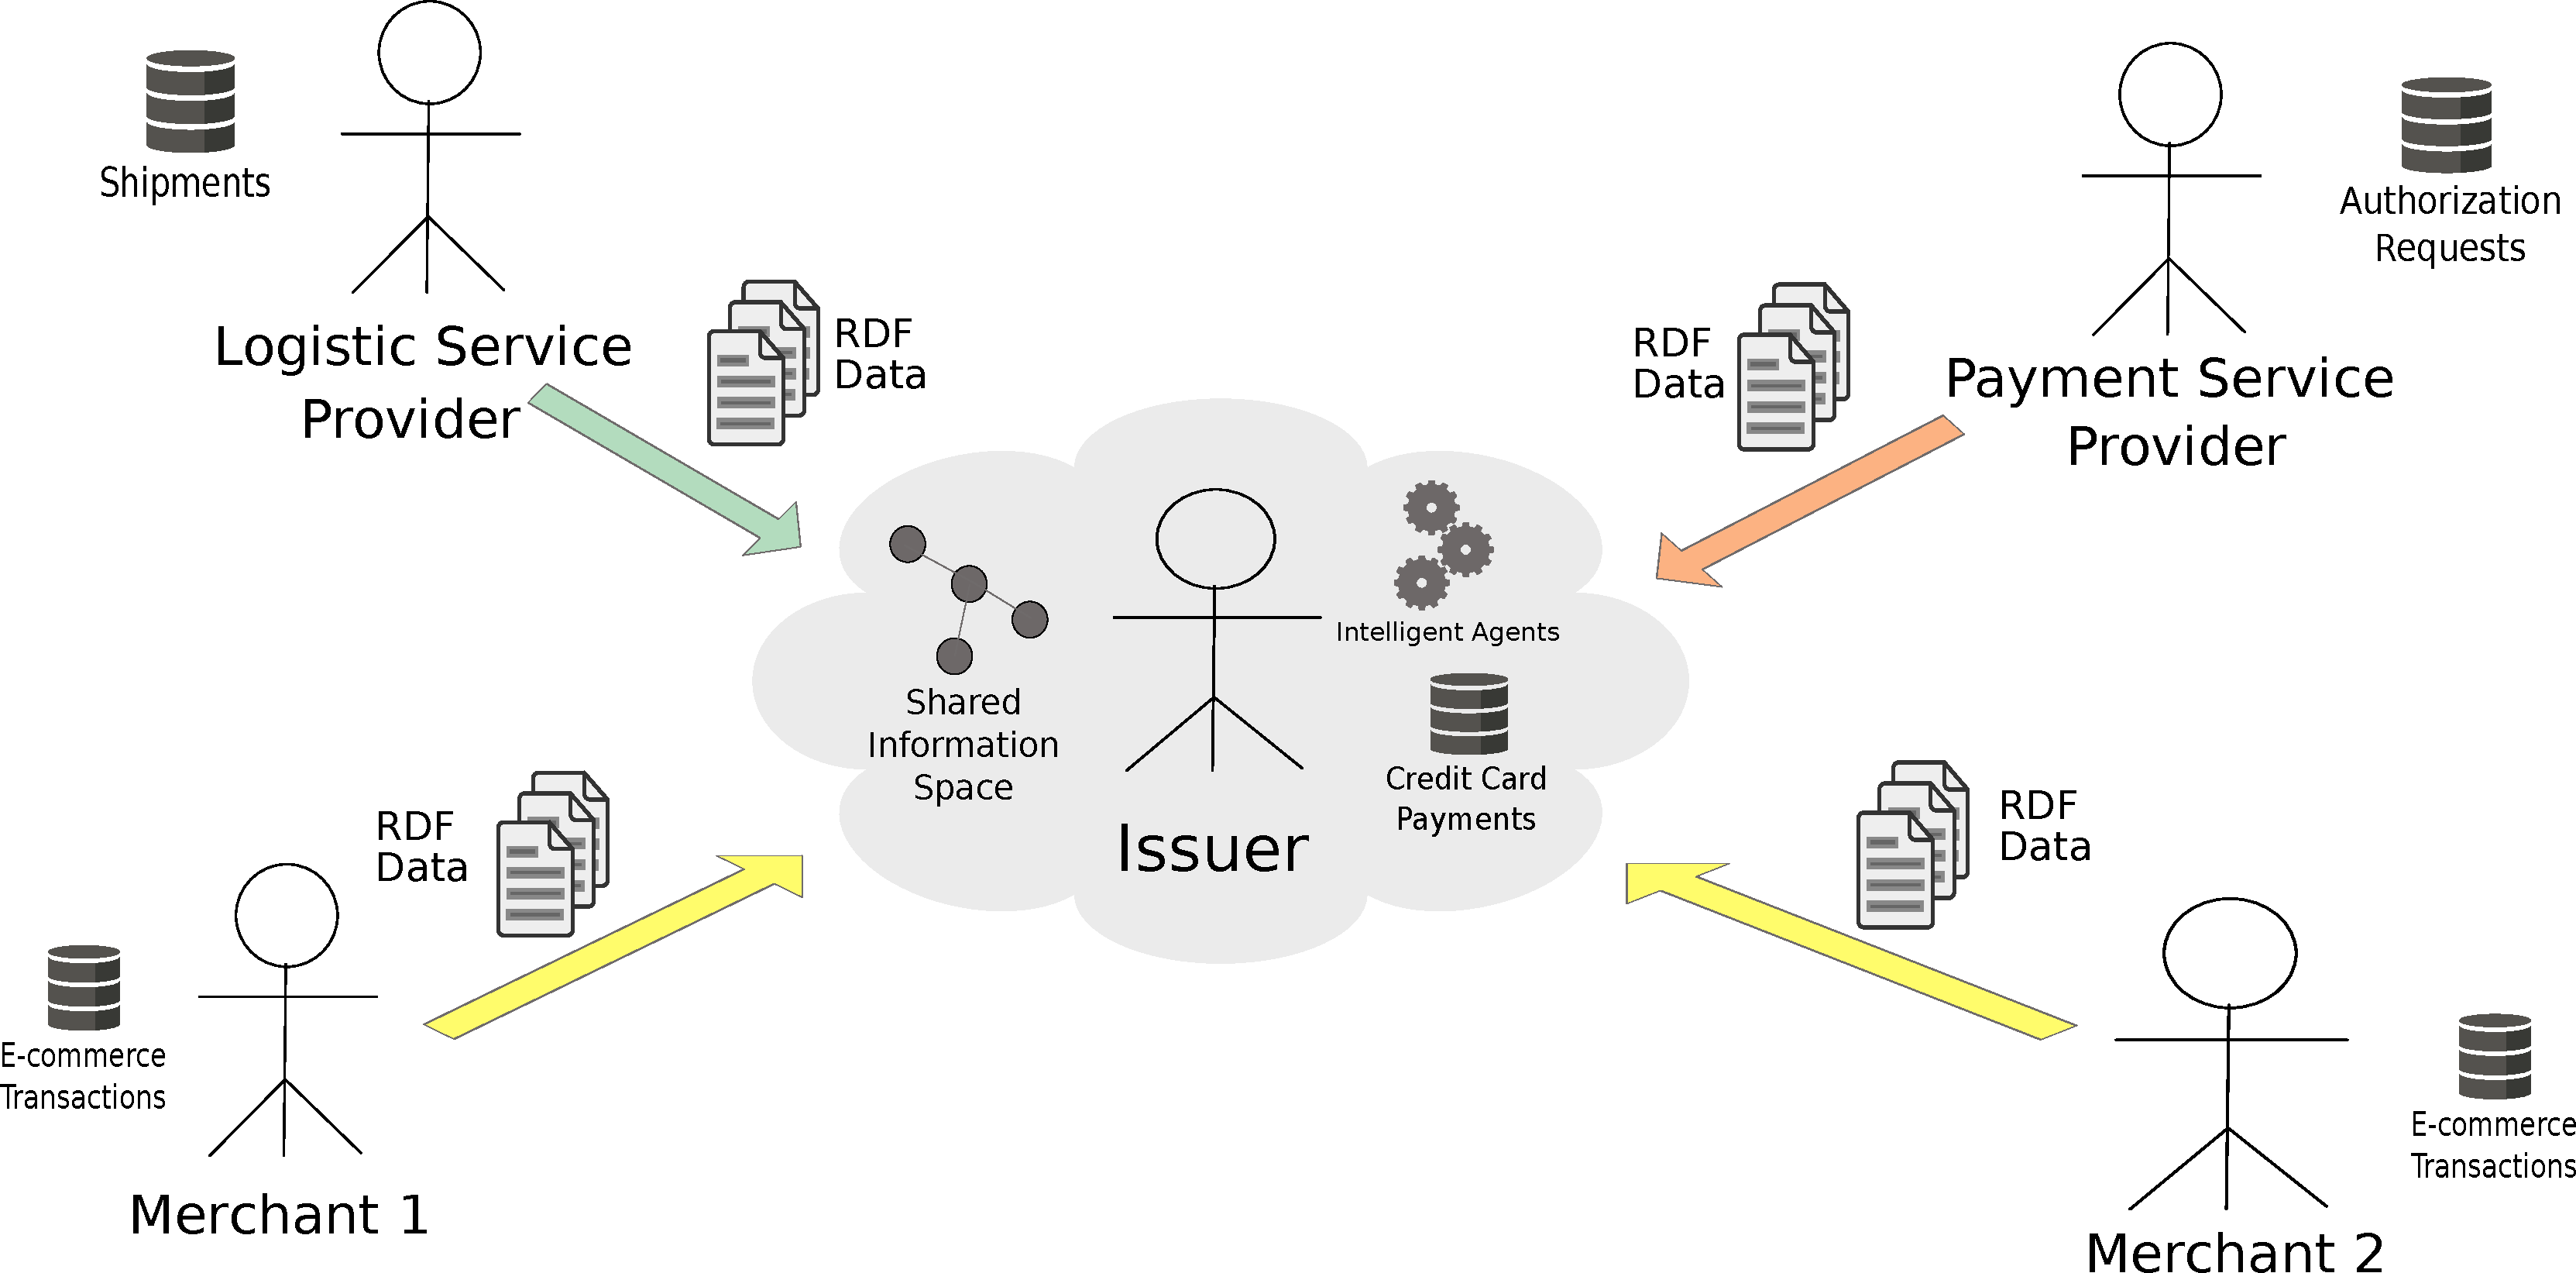
\includegraphics[width=0.8\columnwidth]{images/system_P2P_centralized.pdf}
	\caption{A centralized P2P system design}
\label{fig:images_system_P2P_centralized}
\end{figure}

- a decentralized P2P system in which every node is equal: information is spread over the various nodes; each party holds the information
from the local context (domain specific) and provide an access point incl. API (e.g. SPARQL) for publicly available (shared) content \\
- in this case the intelligent agents can use a mechanism like MapReduce to send the analytics algorithm to the endpoints of the participating parties
and asking for information needed to draw conclusions locally \\

\begin{figure}[H]
	\centering
		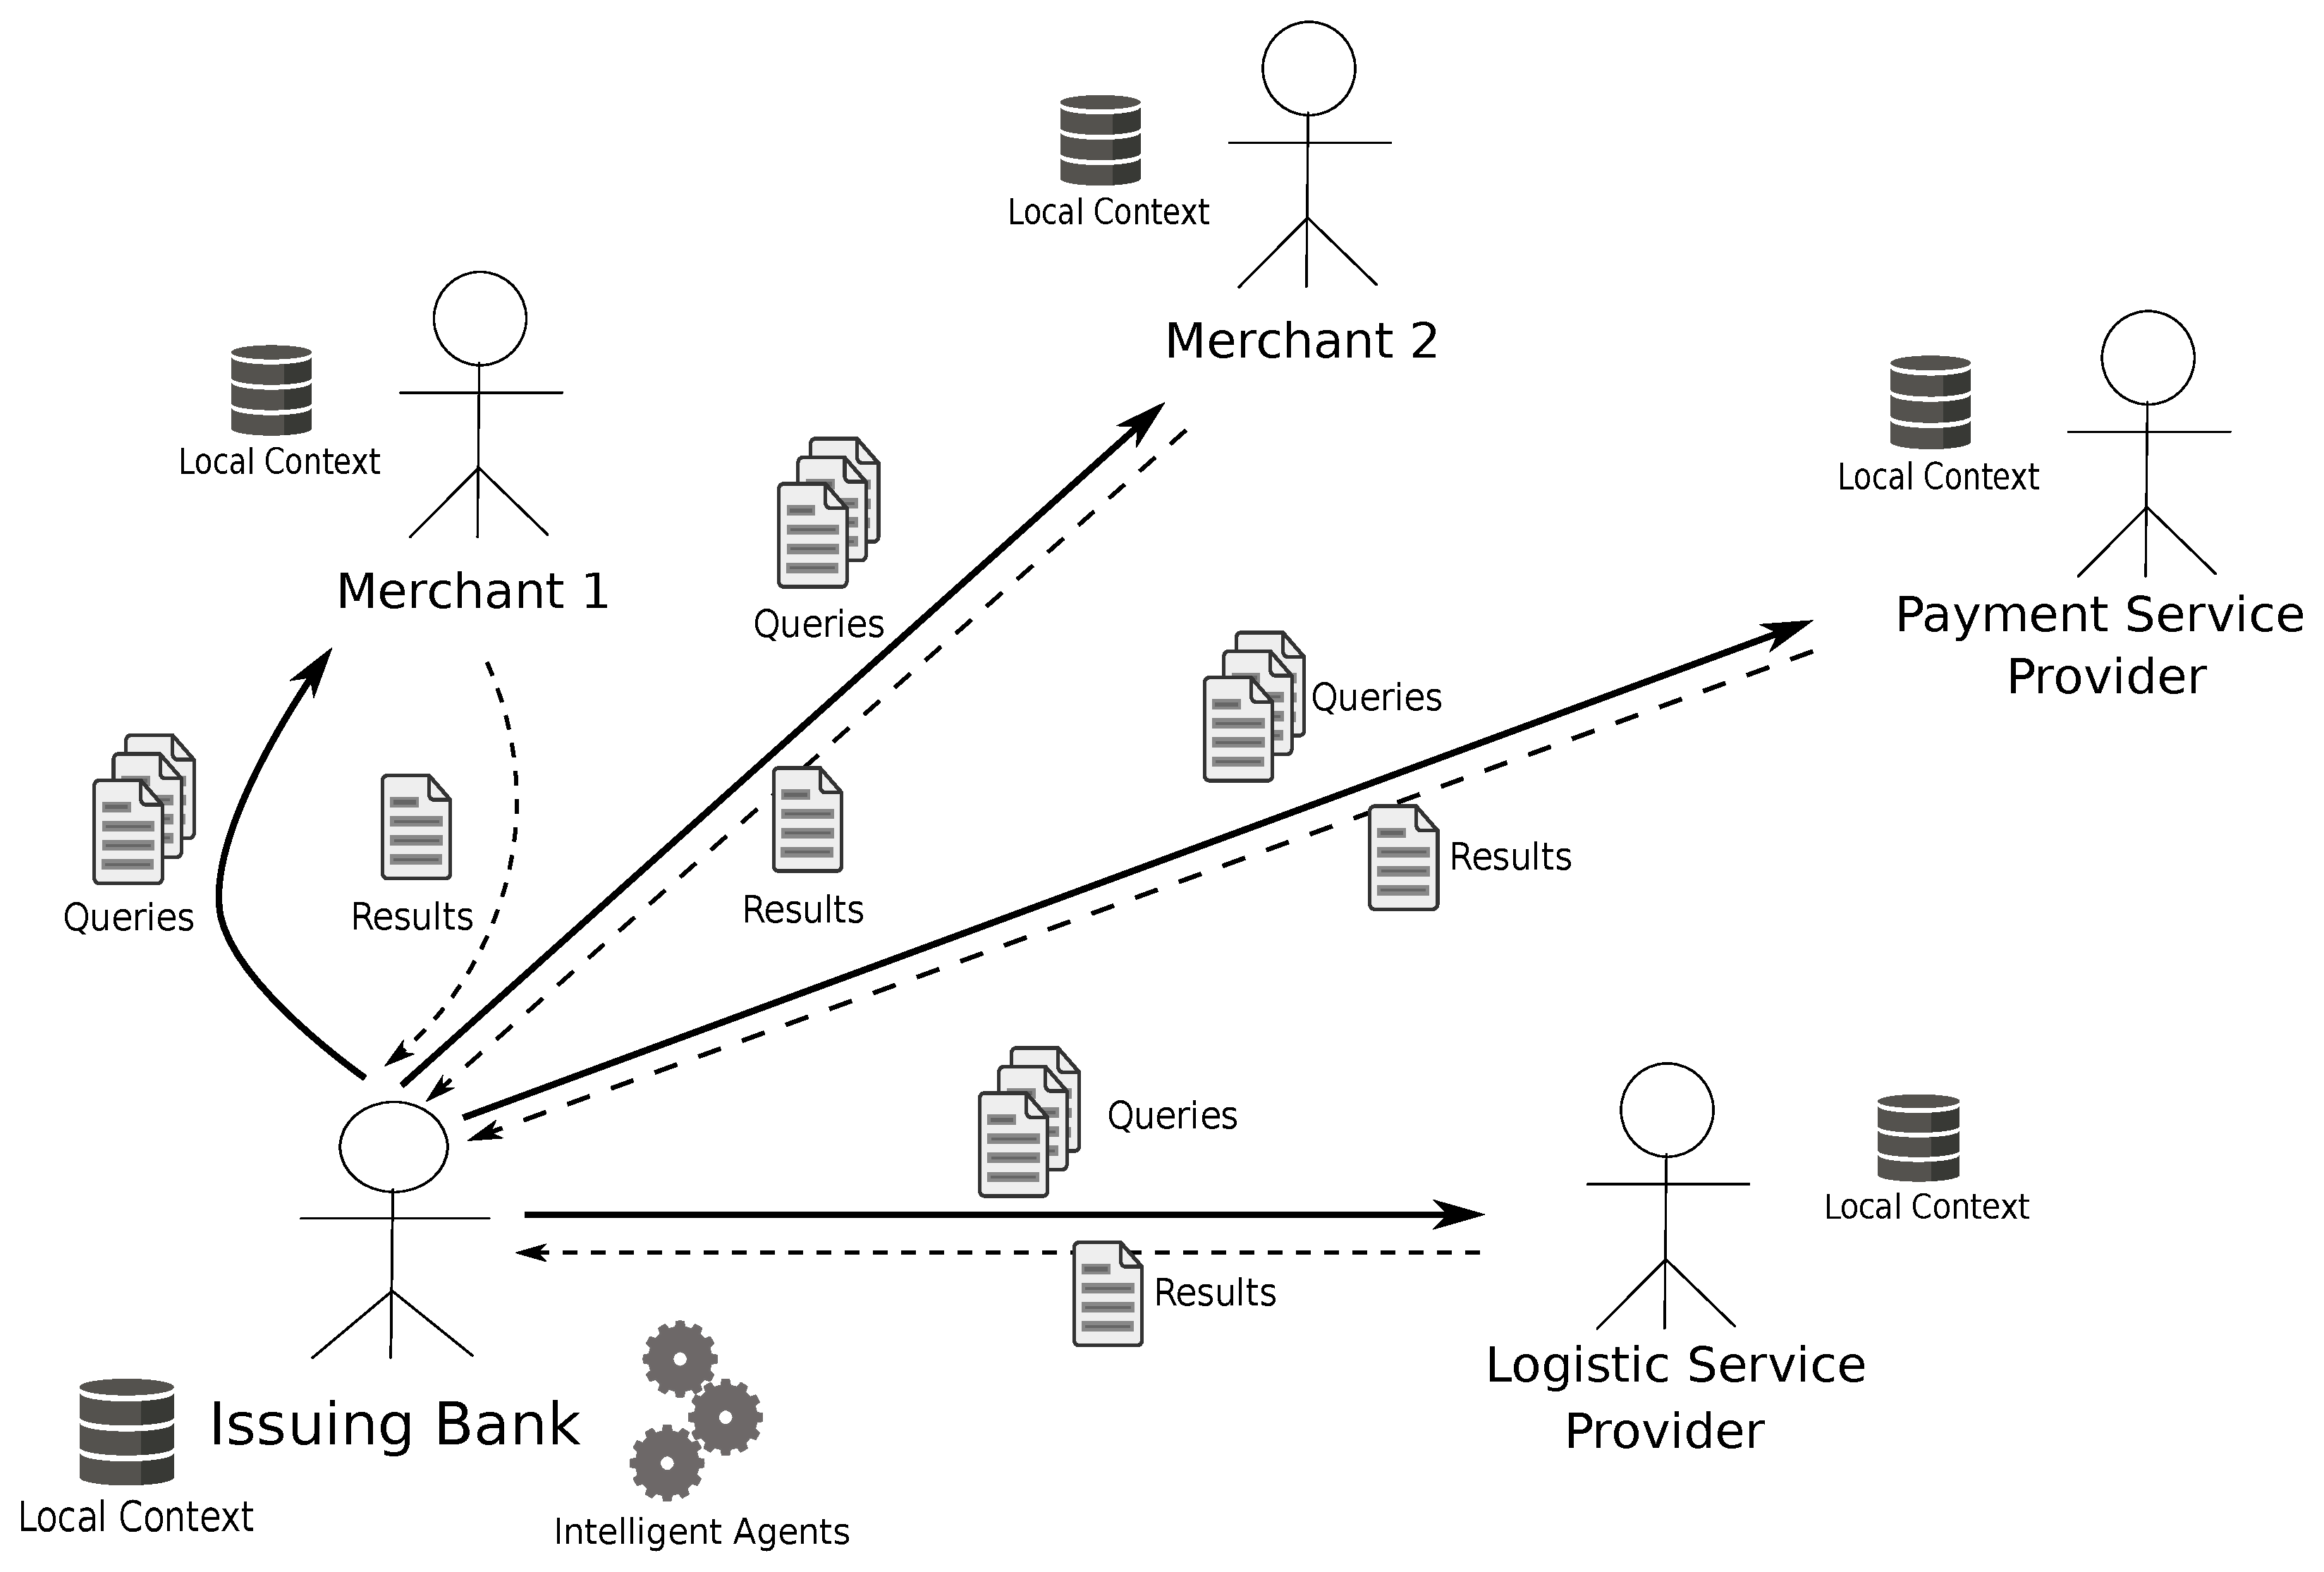
\includegraphics[width=0.8\columnwidth]{images/system_P2P_decentralized.pdf}
	\caption{A decentralized P2P system design}
\label{fig:images_system_P2P_decentralized}
\end{figure}

Reusable Semantic Web resources on the Web: \\
- Ontologies: \\
	1) GoodRelations: describing E-commerce shop transactions \\
	2) Friend-of-a-Friend: describing social relationships between people \\
	3) DublinCore: describing artefacts found on the Web 2.0 (author, date, license, ...) \\
	4) Web Of Trust: describing trust related entities for Web documents (PGP infrastructure) \\
- Sites: \\
  1) DAML: finding ontologies or taxonomies for various domains \\
	2) UMBEL: integrating and mapping technologies and vocabularies for ontologies \\
	3) Wikidata: a free knowledge base representing information from Wikipedia as RDF \\
\\
% chapter design system (end)
